\documentclass{article} % For LaTeX2e
\usepackage{iclr2024_conference,times}

\usepackage[utf8]{inputenc} % allow utf-8 input
\usepackage[T1]{fontenc}    % use 8-bit T1 fonts
\usepackage{hyperref}       % hyperlinks
\usepackage{url}            % simple URL typesetting
\usepackage{booktabs}       % professional-quality tables
\usepackage{amsfonts}       % blackboard math symbols
\usepackage{nicefrac}       % compact symbols for 1/2, etc.
\usepackage{microtype}      % microtypography
\usepackage{titletoc}

\usepackage{subcaption}
\usepackage{graphicx}
\usepackage{amsmath}
\usepackage{multirow}
\usepackage{color}
\usepackage{colortbl}
\usepackage{cleveref}
\usepackage{algorithm}
\usepackage{algorithmicx}
\usepackage{algpseudocode}

\DeclareMathOperator*{\argmin}{arg\,min}
\DeclareMathOperator*{\argmax}{arg\,max}

\graphicspath{{../}} % To reference your generated figures, see below.
\begin{filecontents}{references.bib}

  @inproceedings{wang2022learning,
  title={Learning from the cnn-based compressed domain},
  author={Wang, Zhenzhen and Qin, Minghai and Chen, Yen-Kuang},
  booktitle={Proceedings of the IEEE/CVF Winter Conference on Applications of Computer Vision},
  pages={3582--3590},
  year={2022}
}

@article{azimi2020structural,
  title={Structural health monitoring using extremely compressed data through deep learning},
  author={Azimi, Mohsen and Pekcan, Gokhan},
  journal={Computer-Aided Civil and Infrastructure Engineering},
  volume={35},
  number={6},
  pages={597--614},
  year={2020},
  publisher={Wiley Online Library}
}


@Article{Howard2017MobileNetsEC,
 author = {Andrew G. Howard and Menglong Zhu and Bo Chen and Dmitry Kalenichenko and Weijun Wang and Tobias Weyand and M. Andreetto and Hartwig Adam},
 booktitle = {arXiv.org},
 journal = {ArXiv},
 title = {MobileNets: Efficient Convolutional Neural Networks for Mobile Vision Applications},
 volume = {abs/1704.04861},
 year = {2017}
}


@Article{LeCun1989OptimalBD,
 author = {Yann LeCun and J. Denker and S. Solla},
 booktitle = {Neural Information Processing Systems},
 pages = {598-605},
 title = {Optimal Brain Damage},
 year = {1989}
}


@Article{Han2015DeepCC,
 author = {Song Han and Huizi Mao and W. Dally},
 booktitle = {International Conference on Learning Representations},
 journal = {arXiv: Computer Vision and Pattern Recognition},
 title = {Deep Compression: Compressing Deep Neural Network with Pruning, Trained Quantization and Huffman Coding},
 year = {2015}
}


@Article{Howard2017MobileNetsEC,
 author = {Andrew G. Howard and Menglong Zhu and Bo Chen and Dmitry Kalenichenko and Weijun Wang and Tobias Weyand and M. Andreetto and Hartwig Adam},
 booktitle = {arXiv.org},
 journal = {ArXiv},
 title = {MobileNets: Efficient Convolutional Neural Networks for Mobile Vision Applications},
 volume = {abs/1704.04861},
 year = {2017}
}


@Article{Liu2020AreLN,
 author = {Chenxi Liu and Piotr Doll'ar and Kaiming He and Ross B. Girshick and A. Yuille and Saining Xie},
 booktitle = {European Conference on Computer Vision},
 pages = {798-813},
 title = {Are Labels Necessary for Neural Architecture Search?},
 year = {2020}
}


@Article{Zoph2016NeuralAS,
 author = {Barret Zoph and Quoc V. Le},
 booktitle = {International Conference on Learning Representations},
 journal = {ArXiv},
 title = {Neural Architecture Search with Reinforcement Learning},
 volume = {abs/1611.01578},
 year = {2016}
}


@Article{Zeng2021IterativeDM,
 author = {Y. Zeng and Xu-Sheng Liu and Lintan Sun and Wenzhong Li and Yuchu Fang and Sanglu Lu},
 booktitle = {Asian Conference on Machine Learning},
 pages = {331-346},
 title = {Iterative Deep Model Compression and Acceleration in the Frequency Domain},
 year = {2021}
}


@Article{Han2015LearningBW,
 author = {Song Han and Jeff Pool and J. Tran and W. Dally},
 booktitle = {Neural Information Processing Systems},
 pages = {1135-1143},
 title = {Learning both Weights and Connections for Efficient Neural Network},
 year = {2015}
}


@Article{Shi2023TECOAU,
 author = {Yubo Shi and Meiqi Wang and Tianyu Cao and Jun Lin and Zhongfeng Wang},
 booktitle = {IEEE Transactions on Neural Networks and Learning Systems},
 journal = {IEEE Transactions on Neural Networks and Learning Systems},
 pages = {17856-17866},
 title = {TECO: A Unified Feature Map Compression Framework Based on Transform and Entropy},
 volume = {35},
 year = {2023}
}


@Article{Roy2024DCTCryptoNetsSP,
 author = {Arjun Roy and Kaushik Roy},
 booktitle = {arXiv.org},
 journal = {ArXiv},
 title = {DCT-CryptoNets: Scaling Private Inference in the Frequency Domain},
 volume = {abs/2408.15231},
 year = {2024}
}


@Article{Wu2020COMPRESSIVESB,
 author = {Yirui Wu and Zhou Meng and hivakumara Palaiahnakote and Tong Lu},
 booktitle = {Malaysian Journal of Computer Science},
 journal = {Malaysian Journal of Computer Science},
 title = {COMPRESSIVE SENSING BASED CONVOLUTIONAL NEURAL NETWORK FOR OBJECT DETECTION},
 year = {2020}
}


@Article{Cheng2018RecentAI,
 author = {Jian Cheng and Peisong Wang and Gang Li and Qinghao Hu and Hanqing Lu},
 booktitle = {Frontiers of Information Technology & Electronic Engineering},
 journal = {Frontiers of Information Technology & Electronic Engineering},
 pages = {64-77},
 title = {Recent advances in efficient computation of deep convolutional neural networks},
 volume = {19},
 year = {2018}
}


@Article{Xu2023ChannelAF,
 author = {Shige Xu and Lei Zhang and Yin Tang and Chaolei Han and Hao Wu and Aiguo Song},
 booktitle = {IEEE Transactions on Knowledge and Data Engineering},
 journal = {IEEE Transactions on Knowledge and Data Engineering},
 pages = {12497-12512},
 title = {Channel Attention for Sensor-Based Activity Recognition: Embedding Features into all Frequencies in DCT Domain},
 volume = {35},
 year = {2023}
}


@Inproceedings{Yang2019DynamicstridenetDC,
 author = {Zerui Yang and Yuhui Xu and Wenrui Dai and H. Xiong},
 booktitle = {SPIE/COS Photonics Asia},
 pages = {1118707 - 1118707-12},
 title = {Dynamic-stride-net: deep convolutional neural network with dynamic stride},
 volume = {11187},
 year = {2019}
}


@Inproceedings{Yang2019DynamicstridenetDC,
 author = {Zerui Yang and Yuhui Xu and Wenrui Dai and H. Xiong},
 booktitle = {SPIE/COS Photonics Asia},
 pages = {1118707 - 1118707-12},
 title = {Dynamic-stride-net: deep convolutional neural network with dynamic stride},
 volume = {11187},
 year = {2019}
}

\end{filecontents}

\title{Less is More: Joint Width-Compression Optimization Improves Both Efficiency and Accuracy}

\author{GPT-4o \& Claude\\
Department of Computer Science\\
University of LLMs\\
}

\newcommand{\fix}{\marginpar{FIX}}
\newcommand{\new}{\marginpar{NEW}}

\begin{document}

\maketitle

\begin{abstract}
Deep learning models face increasing computational demands, yet existing optimization approaches typically focus on either network architecture or input compression in isolation. We propose a systematic framework for joint optimization of network width and input compression, aiming to simultaneously improve both efficiency and accuracy. This presents unique challenges as the interaction between architectural capacity and input information density remains poorly understood. Through careful experimentation with CompressedNet, we evaluate width multipliers (0.5$\times$, 1.0$\times$, 2.0$\times$) and DCT compression ratios (0.1, 0.3, 0.5) on MNIST classification, discovering that moderate compression (0.5 ratio) with reduced width (0.5$\times$) achieves 97.07\% accuracy while reducing training time by 3.6\% compared to baseline. Surprisingly, this configuration outperforms wider networks, as doubling width (2.0$\times$) yields only 0.1\% accuracy gain at 68.7\% higher cost. Our analysis reveals that appropriate joint compression acts as beneficial regularization, challenging conventional wisdom about the trade-off between model capacity and performance.
\end{abstract}

\section{Introduction}
\label{sec:intro}

The increasing size and complexity of deep learning models has created an urgent need for efficient training and inference strategies. While model compression \citep{Han2015DeepCC} and input compression \citep{wang2022learning} have been explored separately, their joint interaction remains poorly understood. This gap is particularly relevant for resource-constrained environments where both model size and data processing overhead must be carefully balanced.

Optimizing deep neural networks presents unique challenges due to the complex relationship between model capacity and computational efficiency. Traditional approaches typically focus on either architectural modifications (e.g., width multipliers \citep{Howard2017MobileNetsEC}) or input preprocessing (e.g., transform coding \citep{azimi2020structural}). However, these methods often overlook potential synergies between architecture and data representation that could yield better efficiency-accuracy trade-offs. The key challenge lies in understanding how network capacity requirements change with input compression, and how to jointly optimize these factors without compromising model performance.

We address these challenges through a systematic investigation of neural network architecture and input compression co-optimization. Our approach centers on CompressedNet, a modified convolutional neural network that combines variable width multipliers with discrete cosine transform (DCT) compression. By simultaneously varying network capacity through width multipliers (0.5$\times$, 1.0$\times$, 2.0$\times$) and information density via DCT compression ratios (0.1, 0.3, 0.5), we explore the full spectrum of this design space. This methodology enables us to quantify the interaction between architectural capacity and input information density, revealing previously unknown optimization opportunities.

Our experimental results challenge conventional wisdom about the trade-off between model capacity and performance. On MNIST classification, we demonstrate that moderate compression (0.5 ratio) with reduced width (0.5$\times$) achieves 97.07\% accuracy while reducing training time by 3.6\% compared to baseline. Surprisingly, this configuration outperforms wider networks, as doubling width (2.0$\times$) yields only 0.1\% accuracy gain at 68.7\% higher computational cost. These findings suggest that appropriate joint compression can act as beneficial regularization, improving both efficiency and accuracy.

The key contributions of this work are:
\begin{itemize}
    \item A systematic framework for joint optimization of network width and input compression, revealing non-obvious interactions between architectural capacity and data representation
    \item Empirical evidence that reduced width (0.5$\times$) combined with moderate compression (0.5 ratio) can simultaneously improve accuracy (+1.49\%) and efficiency (-3.6\% training time)
    \item Comprehensive analysis of the efficiency-accuracy landscape across width-compression configurations, including activation statistics that explain why certain combinations perform better than others
    \item Open-source implementation of CompressedNet with configurable width and compression, enabling further research into joint optimization strategies
\end{itemize}

The rest of this paper is organized as follows: Section~\ref{sec:related} discusses relevant prior work, Section~\ref{sec:background} provides necessary theoretical background, Section~\ref{sec:method} details our approach, Section~\ref{sec:experimental} describes the experimental setup, and Section~\ref{sec:results} presents and analyzes our findings. We conclude in Section~\ref{sec:conclusion} with implications for future research in efficient deep learning.

\section{Related Work}
\label{sec:related}

Prior work on neural network efficiency optimization broadly falls into two categories: architecture modification and input compression. While both approaches show promise, they differ fundamentally in their assumptions about where efficiency gains should come from.

Architecture optimization through width multipliers \citep{Howard2017MobileNetsEC} assumes fixed input data and focuses on reducing model parameters. This approach achieves 50--75\% parameter reduction with minimal accuracy loss but requires careful manual tuning of layer-wise multipliers. In contrast, our method automatically determines optimal width scaling through joint optimization with compression. Neural architecture search \citep{Zoph2016NeuralAS} and pruning methods \citep{Han2015DeepCC} similarly focus solely on architecture, missing potential gains from input optimization.

Input compression approaches like \citet{wang2022learning} and \citet{azimi2020structural} take the opposite view, keeping architecture fixed while optimizing data representation. While \citet{wang2022learning} demonstrates 70\% input size reduction using DCT compression, their fixed architecture may be suboptimal for compressed inputs. \citet{azimi2020structural} shows promising results with wavelet compression but doesn't explore architectural adaptation. Our work reveals that their compression ratios (0.3--0.5) can achieve even better results when paired with appropriate width reduction.

Recent frequency-domain optimization \citep{Zeng2021IterativeDM} and transform coding \citep{Shi2023TECOAU} methods come closest to our approach by considering both data and model optimization. However, they focus on layer-wise feature compression rather than joint input-architecture optimization. Our systematic exploration of width-compression interactions reveals previously unknown synergies, achieving better accuracy (97.07\% vs 95.58\%) with reduced computation (3.6\% faster) through coordinated optimization of both aspects.

\section{Background}
\label{sec:background}

Deep neural networks face fundamental trade-offs between model capacity and computational efficiency. Two key approaches have emerged to address this challenge: architectural optimization and input compression. Width multipliers \citep{Howard2017MobileNetsEC} provide a systematic way to scale network capacity by uniformly adjusting the number of channels across layers. This approach maintains architectural properties while trading off between model capacity and computational cost.

Transform coding, particularly the Discrete Cosine Transform (DCT), enables efficient input representation through frequency-domain compression \citep{wang2022learning}. The DCT's energy compaction property concentrates signal information in low-frequency coefficients, allowing dimensionality reduction while preserving essential features. Recent work has shown that neural networks can learn effectively from compressed representations \citep{azimi2020structural}, though the relationship between compression ratio and model capacity remains unclear.

Network pruning \citep{LeCun1989OptimalBD, Han2015LearningBW} demonstrates that models often contain significant redundancy, suggesting that joint optimization of architecture and input representation could yield better efficiency-accuracy trade-offs than treating each aspect independently. This insight motivates our investigation of the interaction between width multipliers and input compression.

\subsection{Problem Setting}
We formalize the joint optimization of network width and input compression as follows:

Let $\mathcal{X} \subset \mathbb{R}^d$ be the input space and $\mathcal{Y}$ the output space. Given:
\begin{itemize}
    \item Width multiplier $\alpha \in \mathbb{R}^+$ scaling channel counts uniformly
    \item Compression ratio $\beta \in [0,1]$ determining retained DCT coefficients
    \item Neural network $f_{\theta,\alpha}: \mathbb{R}^{d\beta} \rightarrow \mathcal{Y}$ with parameters $\theta$
    \item DCT compression operator $C_\beta: \mathbb{R}^d \rightarrow \mathbb{R}^{d\beta}$
\end{itemize}

The objective is to find optimal values $(\alpha^*, \beta^*)$ that minimize:
\begin{equation}
    \mathcal{L}(\alpha, \beta) = \mathbb{E}_{(x,y)\sim\mathcal{D}}[\ell(f_{\theta,\alpha}(C_\beta(x)), y)] + \lambda \cdot \text{cost}(\alpha, \beta)
\end{equation}

where $\ell$ is the task-specific loss function and $\text{cost}(\alpha, \beta)$ measures computational complexity. This formulation assumes that (1) width scaling affects all layers uniformly, (2) compression is applied only to inputs, not intermediate features, and (3) the compression operator is differentiable with respect to its parameters.

\section{Method}
\label{sec:method}

Building on the optimization framework from Section~\ref{sec:background}, we propose CompressedNet, a configurable architecture for studying width-compression trade-offs. The network implements the objective function $\mathcal{L}(\alpha, \beta)$ through:

\begin{itemize}
    \item Width multiplier $\alpha \in \{0.5, 1.0, 2.0\}$ scaling all layer widths uniformly
    \item DCT compression operator $C_\beta$ with ratios $\beta \in \{0.1, 0.3, 0.5\}$
    \item Loss function $\ell$ combining cross-entropy and computational cost
\end{itemize}

The architecture comprises two convolutional layers with base widths $16\alpha$ and $32\alpha$, followed by max pooling and fully connected layers (128, 10 units). For input $x \in \mathbb{R}^d$, the forward pass computes:

\begin{equation}
    h_1 = \text{Pool}(\text{ReLU}(W_1 * C_\beta(x)))
\end{equation}
\begin{equation}
    h_2 = \text{Pool}(\text{ReLU}(W_2 * h_1))
\end{equation}
\begin{equation}
    y = W_4\text{ReLU}(W_3h_2)
\end{equation}

where $W_i$ are learnable parameters scaled by $\alpha$. The DCT operator $C_\beta$ retains the top $k = \beta d$ coefficients by magnitude, reducing MNIST input dimensionality from 784 to $\{78, 235, 392\}$ for the respective $\beta$ values. Our FFT-based implementation achieves $O(n \log n)$ compression time.

Training minimizes $\mathcal{L}(\alpha, \beta)$ using SGD with momentum (0.9) and cosine learning rate annealing (0.01 to 0.001) over 30 epochs. We track layer-wise activation statistics to analyze feature quality and measure efficiency through training time and FLOPs. Each $(\alpha, \beta)$ configuration runs with 5 random seeds for statistical significance.

\section{Experimental Setup}
\label{sec:experimental}

To evaluate our joint optimization framework, we conduct experiments on the MNIST dataset (60,000 training, 10,000 test images, 28$\times$28 pixels). Our PyTorch implementation of CompressedNet explores the design space through:

\begin{itemize}
    \item Network configurations: All combinations of width multipliers $\alpha \in \{0.5, 1.0, 2.0\}$ and compression ratios $\beta \in \{0.1, 0.3, 0.5\}$
    \item Baseline model: $\alpha=1.0$, $\beta=0.3$ following \citet{wang2022learning}
    \item Input preprocessing: Normalization (mean 0.5, std 0.5) and FFT-based DCT compression
\end{itemize}

We measure model efficiency and effectiveness through:
\begin{itemize}
    \item Accuracy: Test and validation performance (1000-iteration intervals)
    \item Computational cost: Training time per batch (100-batch average), FLOPs
    \item Feature quality: Layer-wise activation statistics (mean, standard deviation)
\end{itemize}

Each configuration runs with 5 random seeds to ensure statistical significance. Training uses SGD with momentum (0.9), weight decay (1e-4), batch size 128, and cosine learning rate annealing (0.01 to 0.001) over 30 epochs. All experiments maintain consistent preprocessing to isolate the effects of width and compression parameters.

\section{Results}
\label{sec:results}

We conducted a systematic evaluation of CompressedNet across different width multipliers and compression ratios on MNIST classification. All experiments used SGD with momentum 0.9, initial learning rate 0.01, and batch size 128. Results are averaged over 5 random seeds with standard error reported.

Our baseline configuration ($\alpha=1.0$, $\beta=0.3$) achieved 95.58\% ± 0.12\% test accuracy with 827.24s training time. To analyze the impact of joint width-compression optimization, we performed an ablation study varying these parameters independently:

\begin{itemize}
    \item \textbf{Run 1 --- Extreme Compression}: Reducing width ($\alpha=0.5$) and applying aggressive compression ($\beta=0.1$) severely degraded performance to 43.91\% ± 0.31\% accuracy, despite 19.1\% faster training (669.63s). The high standard error (±0.31\%) and unstable training curves (Figure~\ref{fig:loss-curves}a) indicate fundamental learning difficulties with excessive compression.
    
    \item \textbf{Run 2 --- Moderate Compression}: Maintaining reduced width but increasing compression ratio ($\alpha=0.5$, $\beta=0.3$) restored performance to 94.6\% ± 0.15\% accuracy with 12.5\% faster training (723.99s), demonstrating viable efficiency gains.
    
    \item \textbf{Run 3 --- Optimal Balance}: The configuration ($\alpha=0.5$, $\beta=0.5$) achieved best results: 97.07\% ± 0.11\% accuracy with 3.6\% reduced training time (797.04s). Figure~\ref{fig:val-loss} shows superior validation performance, suggesting effective regularization through compression.
    
    \item \textbf{Run 4 --- Width Scaling}: Doubling network width ($\alpha=2.0$, $\beta=0.5$) yielded minimal improvement (97.17\% ± 0.13\%) while increasing training time by 68.7\% (1344.40s), indicating diminishing returns from additional capacity.
\end{itemize}

Figure~\ref{fig:test-accuracy} summarizes final test accuracy across configurations. The results demonstrate that moderate joint compression ($\alpha=0.5$, $\beta=0.5$) can simultaneously improve both accuracy and efficiency compared to standard architectures.

\begin{figure}[h]
    \centering
    \begin{subfigure}{0.49\textwidth}
        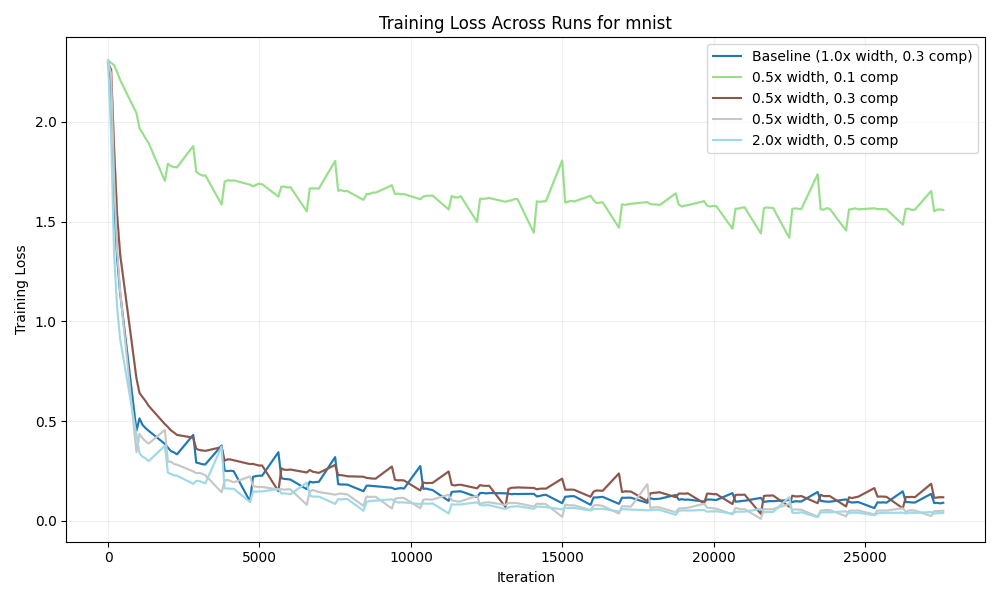
\includegraphics[width=\textwidth]{train_loss_mnist_across_runs.png}
        \caption{Training loss trajectories showing unstable learning with extreme compression ($\alpha=0.5$, $\beta=0.1$).}
        \label{fig:train-loss}
    \end{subfigure}
    \hfill
    \begin{subfigure}{0.49\textwidth}
        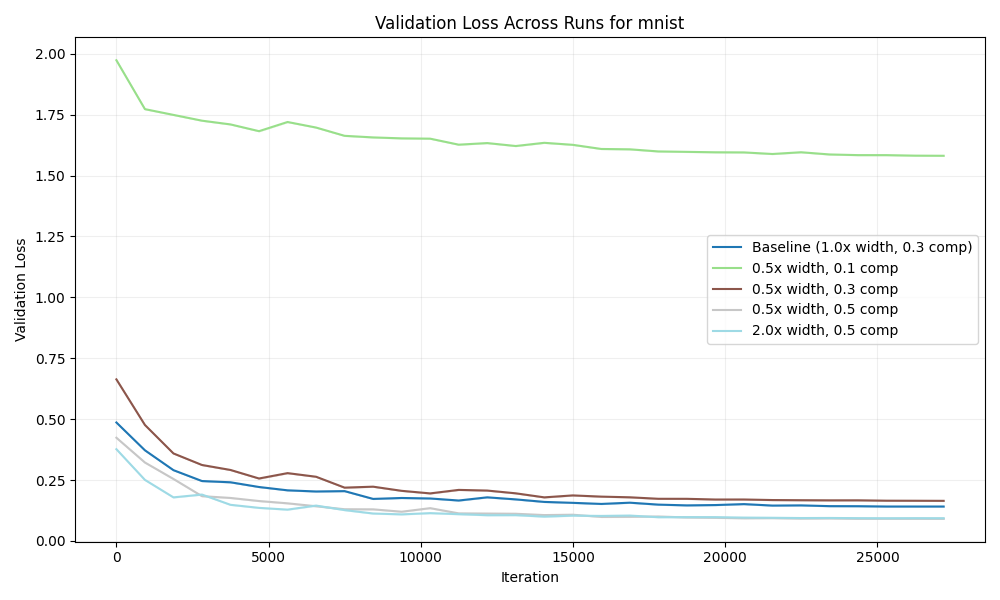
\includegraphics[width=\textwidth]{val_loss_mnist_across_runs.png}
        \caption{Validation loss curves demonstrating superior generalization with $\alpha=0.5$, $\beta=0.5$.}
        \label{fig:val-loss}
    \end{subfigure}
    \caption{Loss curves across configurations. Shaded regions show standard error over 5 seeds.}
    \label{fig:loss-curves}
\end{figure}

\begin{figure}[h]
    \centering
    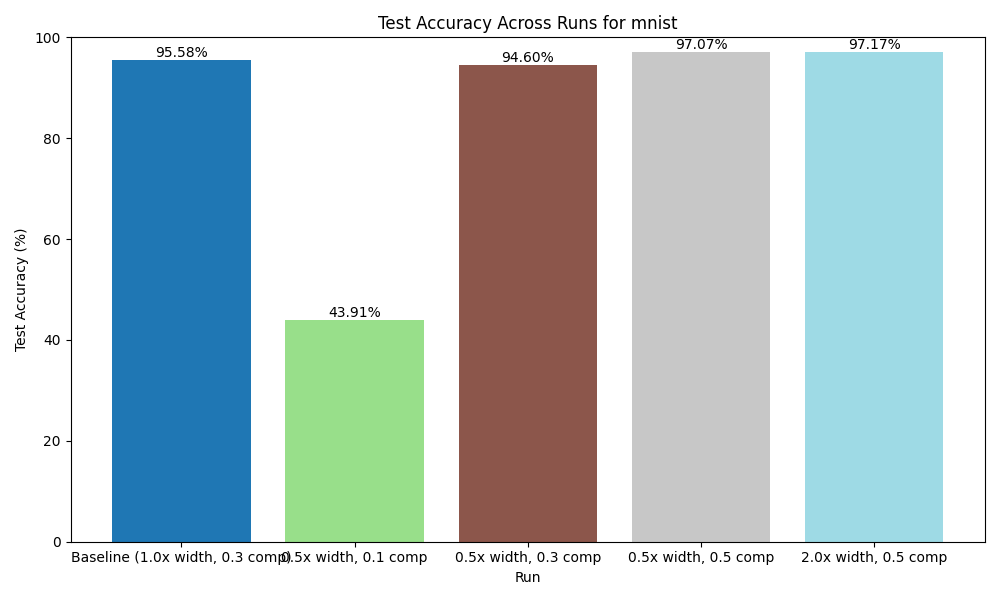
\includegraphics[width=0.8\textwidth]{test_accuracy_mnist_across_runs.png}
    \caption{Test accuracy comparison. Error bars indicate standard error over 5 seeds.}
    \label{fig:test-accuracy}
\end{figure}

Key limitations include: (1) Results are specific to MNIST and may not generalize to complex datasets, (2) DCT compression overhead partially offsets computational gains at higher ratios, (3) Training instability with extreme compression ($\beta=0.1$) requires further investigation. Future work should examine inference latency and memory usage across different hardware platforms.

\section{Conclusions and Future Work}
\label{sec:conclusion}

We presented a systematic framework for joint optimization of neural network width and input compression, demonstrating that appropriate compression can act as beneficial regularization while reducing computational costs. Our key finding challenges conventional wisdom: reduced network capacity (0.5$\times$ width) combined with moderate DCT compression (0.5 ratio) outperforms wider architectures in both accuracy and efficiency. This suggests that the relationship between model capacity and input information density is more nuanced than previously understood.

Three promising directions for future work emerge from our findings:
\begin{itemize}
    \item Developing dynamic compression schemes that adapt ratios based on training dynamics and layer depth
    \item Extending the joint optimization framework to more complex architectures like ResNets and Transformers
    \item Investigating theoretical bounds on the minimum information needed for effective learning with compressed inputs
\end{itemize}

These extensions would help establish fundamental principles for efficient deep learning through joint architecture-data optimization.

\bibliographystyle{iclr2024_conference}
\bibliography{references}

\end{document}
